\documentclass[letterpaper,11pt]{article}

\usepackage[T1]{fontenc}
\usepackage[utf8]{inputenc}
\usepackage[spanish,es-tabla]{babel}
\usepackage{lmodern}
\usepackage[margin=2.5cm,headheight=52pt,headsep=0.3cm]{geometry}
\usepackage{setspace}
\setstretch{1.15}

\usepackage{amsmath}
\usepackage{graphicx}
\usepackage{booktabs}
\usepackage{float}
\usepackage{caption}
\captionsetup{font=small,labelfont=bf,labelsep=colon}
\usepackage{tabularx}
\usepackage{longtable}
\usepackage{array}
\usepackage{enumitem}
\usepackage{csquotes}
\usepackage{tikz}
\usetikzlibrary{positioning,arrows.meta,shapes.geometric,fit}
\usepackage[hidelinks]{hyperref}
\usepackage{fancyhdr}
\usepackage[backend=biber,style=apa]{biblatex}
\DeclareLanguageMapping{spanish}{spanish-apa}

% Las imágenes originales están en documents/entregables/avance/images/.
% El logotipo del template está en esta carpeta.
\graphicspath{ {imagenes/} }
\addbibresource{referencias.bib}

\pagestyle{fancy}
\fancyhf{}
\lhead{Proyecto Integrador}
\rhead{Galaxy Vision}
\cfoot{\thepage}
\renewcommand{\headrulewidth}{0.4pt}
\fancypagestyle{plain}{%
  \fancyhf{}
  \lhead{
\includegraphics[height=1.1cm]{logo.jpeg}}
  \cfoot{\thepage}
  \renewcommand{\headrulewidth}{0pt}
}

\title{\textbf{Clasificación morfológica de galaxias mediante fusión multimodal de imágenes DESI Legacy y espectros integrados MaNGA}}
\author{
Equipo 26: Galaxy Vision\\
Alexander Carreño (A01796955) \quad
María Rabelero (A01793031) \quad
Julio Ricardo Velázquez (A01796953)\\[0.5em]
Proyecto Integrador · Maestría en Inteligencia Artificial Aplicada\\
Asesores: Dr. José Antonio Vázquez Mata y Dr. Héctor Manuel Hernández Toledo\\
Profesora: Dra. Grettel Barceló Alonso
}
\date{11 de noviembre de 2026}

\begin{document}
\maketitle

\begin{abstract}
La clasificación morfológica de galaxias es fundamental para estudiar su formación y evolución, pero requiere de una inspección visual que no es posible escalar con el ritmo de los catálogos astronómicos modernos. Este trabajo desarrolló y comparó modelos que clasifican galaxias como tempranas o tardías a partir de imágenes, espectros integrados y poblaciones estelares derivadas de STARLIGHT. Se integraron etiquetas morfológicas del catálogo de espectros MaNGA, imágenes del DESI Legacy Survey y propiedades de poblaciones estelares derivadas mediante STARLIGHT; después de depurar identificadores y excluir objetos fuera del intervalo definido, se construyó una cohorte estratificada de 9,351 galaxias. El baseline ResNet-18 alcanzó AUC de 0.9633 y exactitud de 0.8881 en el conjunto de prueba. El modelo final seleccionado fue una CNN de cuatro bloques basada únicamente en imágenes: obtuvo AUC de 0.9667 (IC del 95\%: [0.959, 0.975]), exactitud de 0.8952 y exactitud balanceada de 0.8980. Su AUC superó al baseline por 0.0034, una diferencia pequeña frente a la incertidumbre observada; sin embargo, la exactitud aumentó 0.0071. Ambos modelos excedieron los objetivos del proyecto de exactitud 0.829 y F1 0.83. La fusión no mejoró de forma consistente el desempeño. Por ello, se recomienda una solución de imagen como clasificador operativo, con revisión humana de casos inciertos y fuentes espectrales como señales complementarias aún por validar.
\end{abstract}

\noindent\textbf{Palabras clave:} morfología galáctica, aprendizaje profundo, CNN, MaNGA, DESI Legacy Survey, clasificación multimodal.

\section{Contexto de negocio y problema}

\subsection{Necesidad científica y operativa}

La morfología de una galaxia resume rasgos observables que ayudan a investigar su estructura, su población estelar y su historia de evolución. La clasificación visual experta proporciona etiquetas valiosas, pero requiere tiempo y puede ser ambigua, especialmente para objetos compactos, difusos o de baja señal. Los catálogos de gran escala hacen necesario automatizar una parte del proceso sin presentar las predicciones como sustituto de la validación científica.

El proyecto responde a esta necesidad mediante un clasificador binario que prioriza objetos para su análisis. El objetivo operativo es reducir el esfuerzo de revisión manual, manteniendo un desempeño suficientemente alto y haciendo visibles los casos de mayor riesgo. La solución estudiada no constituye todavía un servicio productivo: el trabajo cubrió la exploración, preparación, entrenamiento y evaluación de modelos; el despliegue y el monitoreo continuo quedan como trabajo futuro.

\subsection{Definición del problema y criterio de éxito}

La etiqueta se construyó a partir de \texttt{Ttype}: se asignó la clase temprana (0) si \texttt{Ttype} $\leq 0$ y la clase tardía (1) si $1 \leq \texttt{Ttype} \leq 10$. Los 67 objetos con \texttt{Ttype}=11 quedaron fuera de ese dominio. Esta regla transforma una secuencia morfológica continua en dos categorías y, por tanto, no elimina la ambigüedad de las galaxias cercanas a la frontera entre tipos.

El avance inicial fijó como objetivos mínimos superar una exactitud de 0.829 y un F1 de 0.83, además de conservar un comportamiento adecuado en ambas clases y producir probabilidades utilizables. La métrica principal de comparación entre modelos fue el área bajo la curva ROC (AUC), que mide capacidad de ordenamiento y no depende de un único umbral de decisión. Para evaluar el punto operativo también se informan exactitud, exactitud balanceada, recuperación por clase y F1. La reducción de trabajo de revisión es una meta de negocio; no se midió directamente en un flujo productivo.

\subsection{Evolución del enfoque}

La hipótesis original fue que combinar imágenes y espectros superaría a los clasificadores unimodales. La evidencia no la confirmó. La CNN de imágenes alcanzó el mejor resultado de la última comparación, mientras que algunas fusiones tuvieron AUC inferior y mayor variabilidad de entrenamiento. Por ello, el enfoque finalmente adoptado es un clasificador basado solo en imágenes. Los espectros y las poblaciones estelares se conservan como expertos complementarios potenciales, no como entradas necesarias del modelo operativo.

Esta decisión no implica que la información espectral carezca de valor. El análisis mostró que un modelo de poblaciones puede corregir parte de los errores de imagen. Sin embargo, para aprovechar ese complemento hace falta aprender una regla de selección o combinación usando predicciones fuera de pliegue y validación separada; una selección ideal a posteriori no es implementable sin riesgo de optimismo.

\begin{figure}[H]
  \centering
  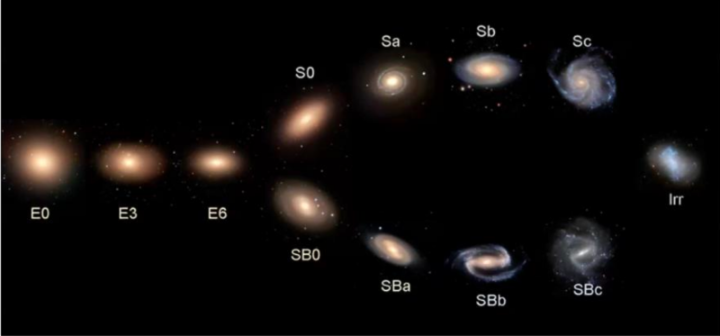
\includegraphics[width=0.85\linewidth]{tipos_galaxias.png}
  \caption{Representación ilustrativa de tipos morfológicos galácticos. La clasificación binaria del proyecto comprime un continuo de estructuras en dos clases.}
  \label{fig:tipos}
\end{figure}

\section{Datos y preparación}

\subsection{Fuentes, integración y etiquetas}

El proyecto integró el catálogo de morfología visual MaNGA con imágenes de DESI Legacy Survey y espectros integrados MaNGA. Los patrocinadores científicos del proyecto participan en el trabajo de morfología visual MaNGA; ello aporta contexto experto, pero no elimina la necesidad de validar la representatividad y consistencia de las etiquetas. Los espectros de MaNGA permiten caracterizar propiedades físicas y poblacionales, mientras que la imagen presenta directamente la estructura proyectada del objeto \parencite{bundy2015, dey2019, vazquezmata2022}.

El catálogo inicial contenía 10,126 filas y nueve variables, sin duplicados. Se observaron 33 valores faltantes en \texttt{PETRO\_TH90}, 28 en \texttt{LogMass} y uno en \texttt{nsa\_z}; además, 27 filas tenían \texttt{nsa\_z} con el valor centinela $-9999$. El tipo morfológico cubría 50 subclases y la etiqueta binaria estaba desbalanceada: 6,385 tardías (63.1\%) y 3,741 tempranas (36.9\%). Tras depuración, el catálogo curado reunió 10,014 galaxias: 6,292 tardías y 3,722 tempranas.

La inspección de identificadores encontró 10,243 archivos FITS espectrales: 10,013 coincidían con el catálogo, una galaxia catalogada no tenía FITS y 230 espectros no tenían entrada en el catálogo. La cohorte utilizada en los experimentos tuvo 9,351 galaxias y se dividió una sola vez, con semilla 42 y estratificación, en entrenamiento, validación y prueba (70/15/15). Las diferencias entre el tamaño curado y la cohorte experimental reflejan la disponibilidad de los insumos usados por esos experimentos.

\begin{table}[H]
\centering
\caption{Distribución de clases en la cohorte experimental.}
\label{tab:split}
\begin{tabular}{lrrrr}
\toprule
Partición & Total & Tardías & Tempranas & Proporción tardías\\
\midrule
Entrenamiento & 6,545 & 4,078 & 2,467 & 62.3\%\\
Validación & 1,403 & 874 & 529 & 62.3\%\\
Prueba & 1,403 & 875 & 528 & 62.4\%\\
\midrule
Total & 9,351 & 5,827 & 3,524 & 62.3\%\\
\bottomrule
\end{tabular}
\end{table}

\subsection{Preparación de imágenes}

Se procesaron imágenes grz en recortes de $256 \times 256$ píxeles. El campo de visión se definió en relación con \texttt{PETRO\_TH90}, con variantes entre cuatro y ocho veces esa escala y siete variantes de campo de visión para todos los objetos de la cohorte. La elección adaptativa responde a la gran dispersión del tamaño angular: la mediana de \texttt{PETRO\_TH90} fue 13 segundos de arco y el máximo, 148. Se aplicaron rotaciones de 0, 90, 180 y 270 grados, además de volteos horizontal y vertical, exclusivamente durante el entrenamiento.

La inspección de una muestra de cubos FITS encontró arreglos de tres canales de tamaño $256 \times 256$, tipo \texttt{float32} y sin valores NaN. Los cubos estaban verticalmente invertidos respecto de la imagen de referencia: corregir la orientación elevó la correlación de 0.73 a 0.98. Las unidades originales eran nanomaggies por píxel nativo de 0.262 segundos de arco. También se identificó un posible efecto de región: el color $r-z$ predecía norte/sur con AUC 0.712. La visualización de los FITS redujo la diferencia cromática norte/sur frente a JPEG de 0.134 a 0.044, pero el riesgo de fuga por región y por representación de imagen no queda descartado.

\begin{figure}[H]
  \centering
  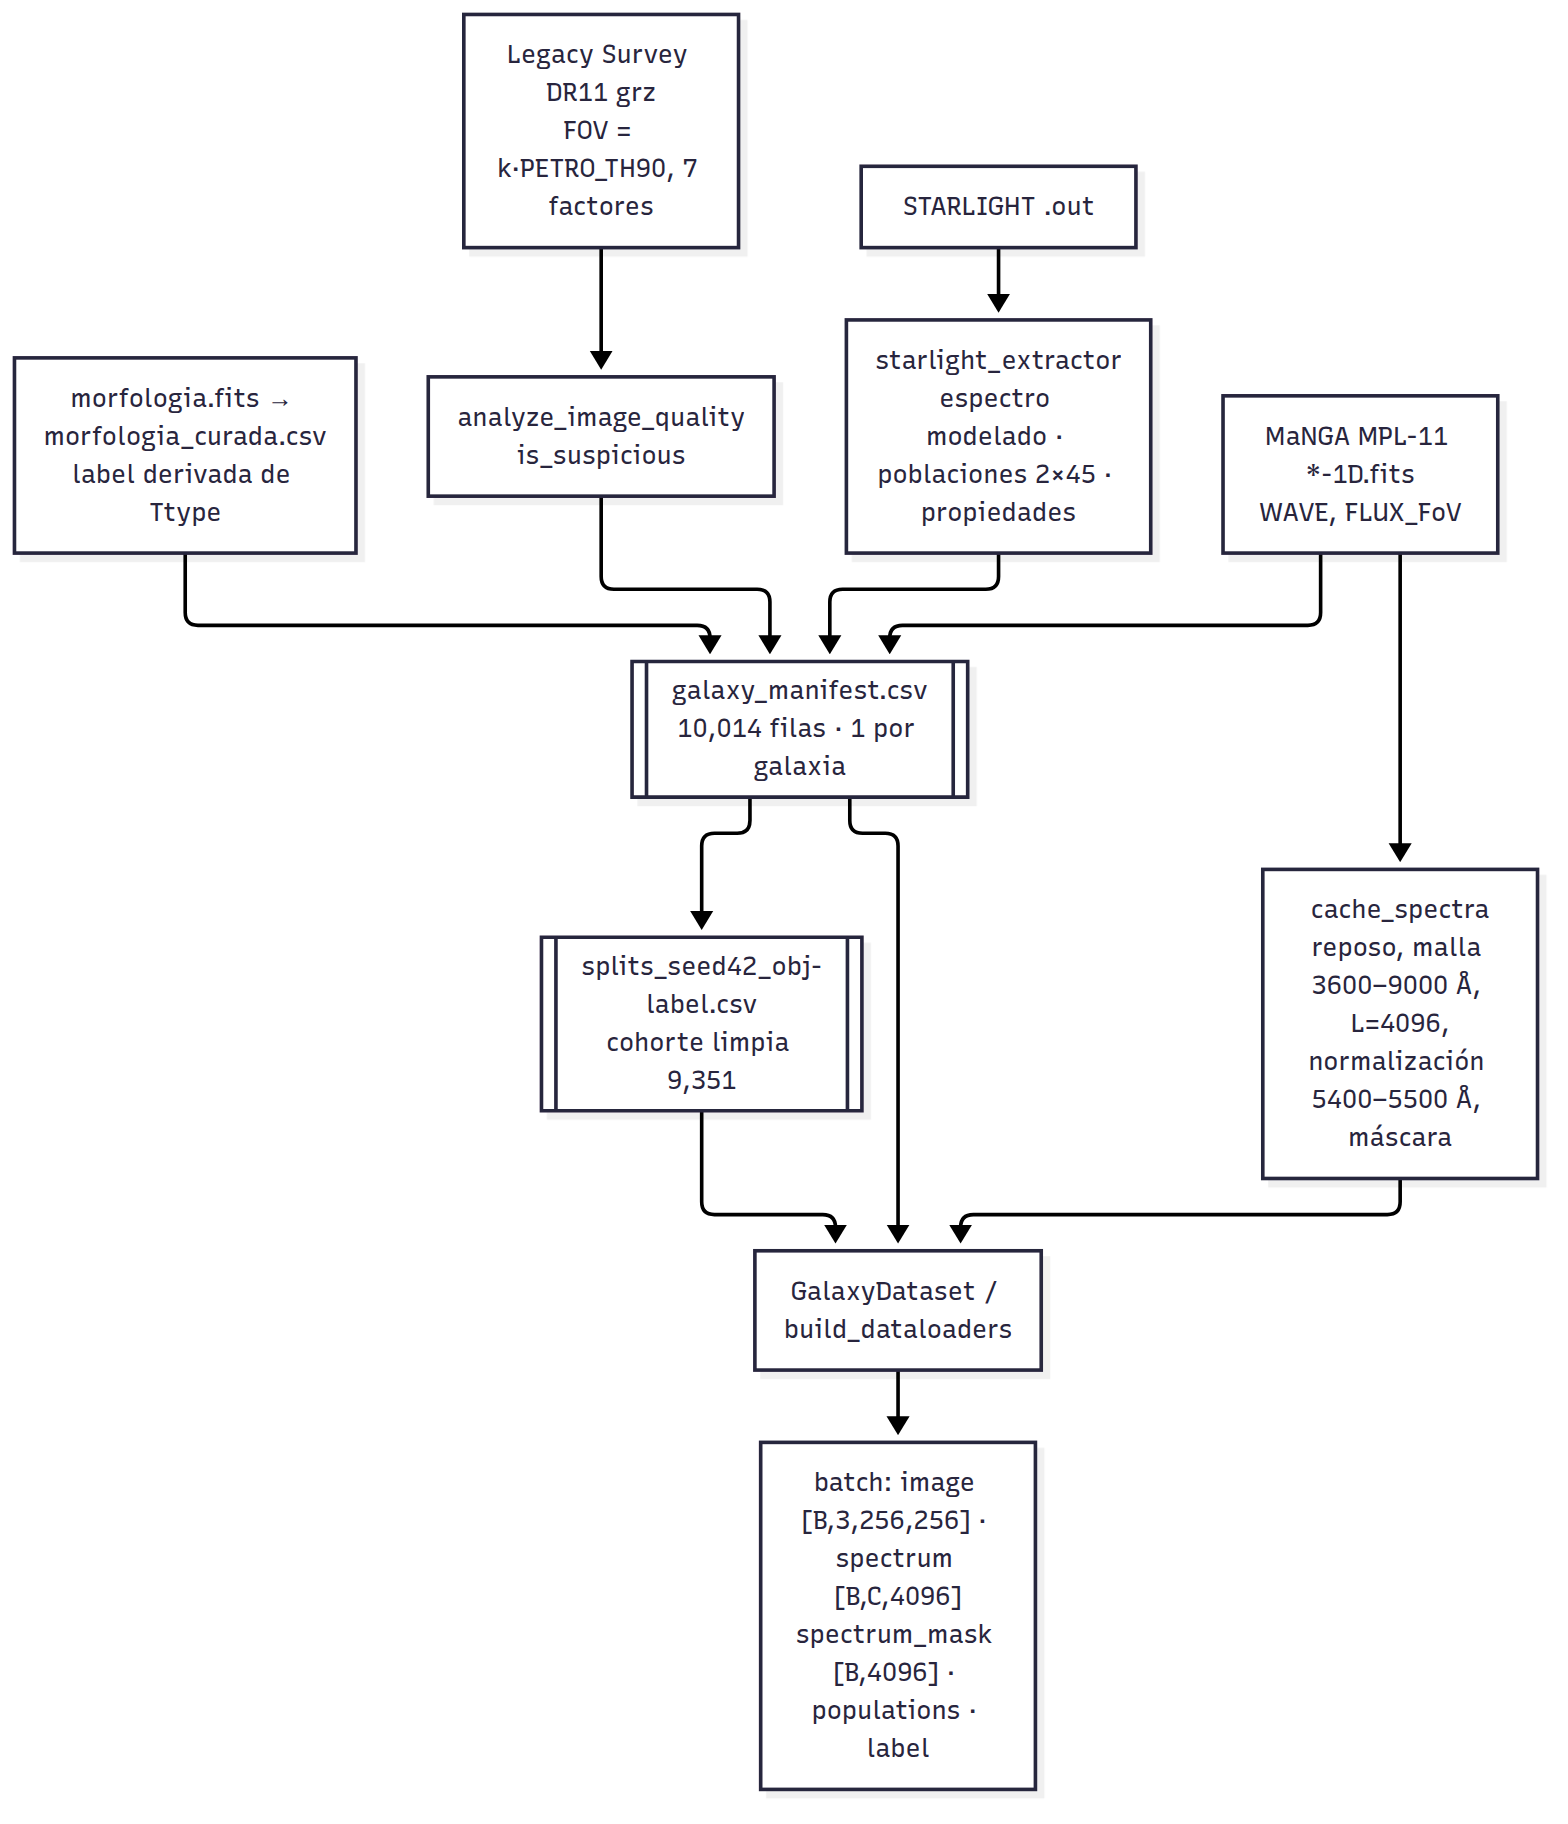
\includegraphics[width=0.92\linewidth]{diag3_flujo_datos.png}
  \caption{Flujo de integración y preparación de los datos. La selección de la cohorte, la orientación y el tamaño del recorte son parte del contrato de datos del modelo.}
  \label{fig:flujo}
\end{figure}

\subsection{Espectros, metadatos y prevención de fugas}

Los espectros se transformaron al marco de reposo mediante $\lambda/(1+z)$, se normalizaron con la mediana en el intervalo 5400--5500 \AA{} y se interpolaron a una malla de 4,096 muestras entre 3600 y 9000 \AA{}, sin extrapolación. Las posiciones sin cobertura se representaron mediante relleno con ceros y una máscara espectral. Para un muestreo exploratorio de 300 espectros se reportaron 4,487 puntos originales entre 3622 y 10351 \AA{} y una mediana provisional de relación señal-ruido cercana a 311.

Las variables numéricas de metadatos se imputaron y normalizaron usando únicamente estadísticas del conjunto de entrenamiento. Se prohibió usar como entradas la etiqueta, \texttt{Ttype}, \texttt{Type}, nombre, ascensión recta y declinación. Esto reduce la posibilidad de que el modelo memorice identificadores o codifique directamente la respuesta. Las fracciones poblacionales STARLIGHT suman 90 variables (45 fracciones de luz y 45 de masa, basadas en BC03); como se derivan de los mismos espectros FLUX\_FoV, no son una fuente independiente de evidencia.

La calidad de imagen también limita la interpretación. En una inspección de 1,000 galaxias DR11, 1.9\% tenía \texttt{line\_flag}, 27.6\% \texttt{bright\_flag} y 27.7\% \texttt{is\_suspicious}. La exactitud reportada describe el conjunto evaluado, no garantiza el mismo desempeño tras excluir o incorporar otros niveles de calidad.

\section{Metodología y modelos}

\subsection{Protocolo experimental}

Se siguió una secuencia de desarrollo inspirada en CRISP-ML(Q): definir el problema y los criterios de aceptación; comprender y preparar los datos; entrenar modelos; y evaluar sus resultados. No se completaron las fases de despliegue y monitoreo como operación real. La partición de prueba se mantuvo fija para las comparaciones de los avances, pero el proceso usó una sola semilla y una sola división. Por tanto, las diferencias pequeñas entre modelos no deben interpretarse como evidencia concluyente de superioridad poblacional.

\subsection{Baseline: ResNet-18 de imágenes}

El primer baseline fue una ResNet-18 inicializada desde cero. Su representación de 512 dimensiones se proyectó a un embedding de 128 dimensiones y a un perceptrón multicapa de clasificación. Se usaron AdamW, tasa de aprendizaje $10^{-4}$, decaimiento de peso $10^{-4}$ y pérdida \texttt{BCEWithLogits}. El entrenamiento aplicó parada temprana con paciencia de ocho épocas y terminó en la época 32; la mejor AUC de validación fue 0.9644 en la época 24.

En prueba, el baseline obtuvo AUC 0.9633 y exactitud 0.8881. La exactitud balanceada fue 0.8825 y el F1 macro 0.8812. La matriz de confusión, con filas de clase real temprana/tardía y columnas de predicción temprana/tardía, fue
\[
\begin{pmatrix}
454 & 74\\
83 & 792
\end{pmatrix}.
\]
En otras palabras, clasificó correctamente 454 de 528 galaxias tempranas y 792 de 875 tardías. Su intervalo bootstrap del 95\% para AUC fue [0.955, 0.972]. La brecha entre exactitud de entrenamiento (0.9337), validación (0.8959) y prueba (0.8881), junto con pérdidas finales de 0.159 y 0.317 para entrenamiento y validación, respectivamente, indicó sobreajuste. Se reportaron ECE de 0.038 y Brier de 0.077.

\subsection{Candidatos y evidencia multimodal}

Los experimentos siguientes compararon una CNN de cuatro bloques, imágenes con campos de visión aleatorios, espectros procesados con CNN 1D o RNN, fracciones STARLIGHT y varias fusiones. La CNN compacta de imágenes, con aproximadamente 1.2 millones de parámetros, alcanzó exactitud 0.9009 y AUC entre 0.9623 y 0.9643 en las primeras corridas comparativas. Las variantes imagen-espectro y las de poblaciones no mostraron una mejora estable sobre la imagen sola. La fusión de imagen, espectro y poblaciones llegó a AUC 0.9650 en una corrida, pero su incremento de 0.0017 sobre ResNet-18 fue menor que el error estándar aproximado de 0.005 y la exactitud fue 0.8895.

En el estudio de espectros de Avance 5, \texttt{patch\_bigru} obtuvo AUC 0.9170 (IC del 95\%: [0.901, 0.931]), exactitud 0.8525 y 203,009 parámetros. \texttt{cnn\_bigru} alcanzó 0.9122 y la CNN 1D de referencia 0.8572 (IC del 95\%: [0.837, 0.877]). La mejora frente a la referencia no puede atribuirse únicamente a la recurrencia: también cambiaron la capacidad y la optimización. Estos resultados sitúan las variantes espectrales en un rango de AUC aproximado de 0.90--0.92, por debajo de las mejores imágenes para esta tarea y partición.

\subsection{Modelo final: CNN de imágenes}

El modelo final fue \texttt{image\_only\_control}, una CNN de cuatro bloques con 1,222,753 parámetros. Se entrenó con tasa de aprendizaje $3 \times 10^{-4}$, clipping de gradiente 1.0 y un máximo de 50 épocas; la mejor época fue la 47. En el conjunto de prueba obtuvo AUC 0.9667 (IC del 95\%: [0.959, 0.975]), exactitud 0.8952 y exactitud balanceada 0.8980. La recuperación fue 0.909 para tempranas y 0.887 para tardías; el F1 tardío fue 0.9135 y la pérdida de prueba 0.2489.

El resultado de fusión más reciente, CNN de imágenes con atención sobre espectros, obtuvo AUC 0.9334, exactitud 0.8617 y exactitud balanceada 0.8696; su mejor época fue la 4 de 12. En comparación pareada, la diferencia de AUC fusión menos modelo de imagen fue $-0.0333$ (IC [-0.0447, -0.0227]). La evidencia favorece la decisión de desplegar inicialmente la CNN de imágenes, no la fusión. El patrón no demuestra que la modalidad espectral sea inútil: demuestra que las fusiones implementadas no aprendieron una combinación que superara al control visual en esta evaluación.

\begin{figure}[H]
  \centering
  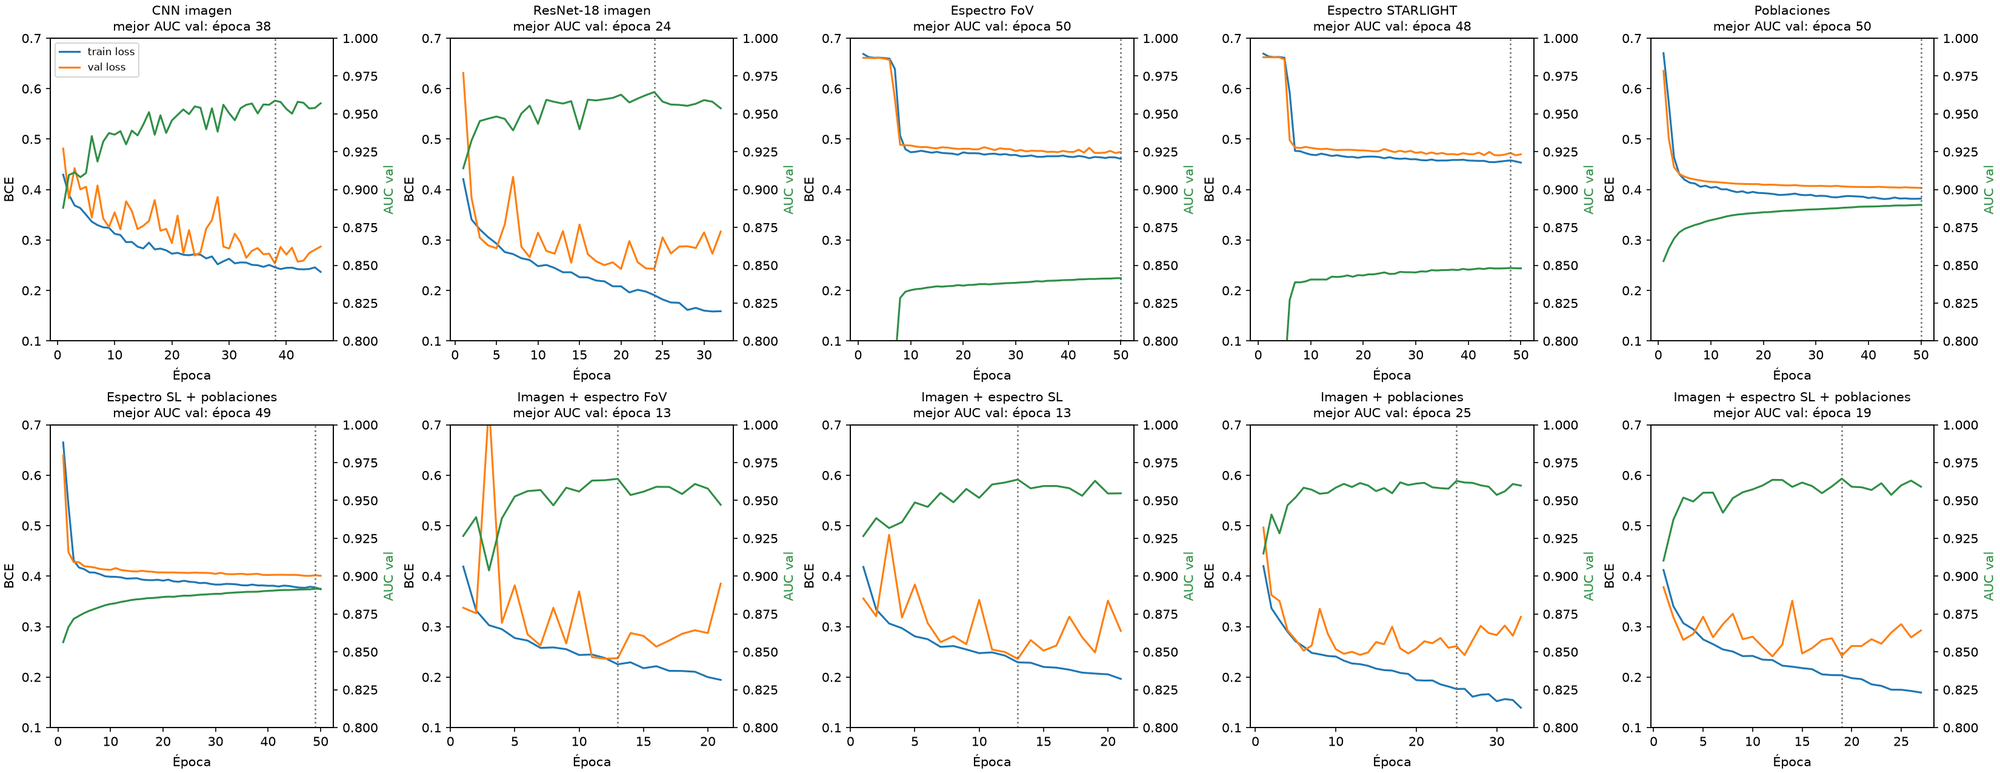
\includegraphics[width=0.78\linewidth]{curvas_entrenamiento.png}
  \caption{Curvas de entrenamiento de modelos candidatos. La selección se basó en validación; las curvas también permiten identificar divergencias compatibles con sobreajuste.}
  \label{fig:curvas}
\end{figure}

\section{Resultados y validación}

\subsection{Comparación con baseline y objetivos}

La diferencia del modelo final respecto al baseline es de +0.0034 AUC (0.9667 frente a 0.9633), +0.0071 de exactitud (0.8952 frente a 0.8881) y +0.0155 de exactitud balanceada (0.8980 frente a 0.8825). La diferencia de AUC es pequeña y los intervalos de confianza se solapan; con una única partición no debe describirse como una mejora estadísticamente estable. La exactitud, por su parte, sí aumentó en el conjunto de prueba observado. El modelo compacto reportó además ECE 0.014 y Brier 0.072 en su evaluación de calibración, frente a 0.038 y 0.077 del baseline; la comparación de calibración debe interpretarse con cautela si no se replica con el mismo protocolo y particiones.

\begin{table}[H]
\centering
\caption{Desempeño de referencia, modelo final y objetivos del proyecto en prueba.}
\label{tab:resultados}
\begin{tabularx}{\linewidth}{>{\raggedright\arraybackslash}Xrrrr}
\toprule
Modelo / criterio & AUC & Exactitud & Exactitud balanceada & F1 reportado\\
\midrule
Objetivo mínimo & -- & 0.829 & -- & 0.83\\
Baseline ResNet-18 & 0.9633 & 0.8881 & 0.8825 & 0.8812 macro\\
CNN final de imágenes & \textbf{0.9667} & \textbf{0.8952} & \textbf{0.8980} & 0.9135 tardía\\
\midrule
Cambio final vs. baseline & +0.0034 & +0.0071 & +0.0155 & no equivalente\\
Brecha final vs. objetivo & -- & \textbf{+0.0662} & -- & \textbf{+0.0835*}\\
\bottomrule
\end{tabularx}

\vspace{0.3em}
\footnotesize{* La brecha de F1 compara el F1 de la clase tardía reportado para el modelo final con el umbral de 0.83 del proyecto. No es estrictamente equivalente al F1 macro del baseline ni a un F1 global sin especificación de promedio.}
\end{table}

La exactitud final excedió el mínimo de 0.829 por 0.0662, es decir, 6.62 puntos porcentuales. El F1 tardío de 0.9135 queda 0.0835 por encima del criterio numérico de 0.83, con la salvedad de que el umbral inicial no especifica el promedio de F1. El baseline también superó los umbrales: exactitud por 0.0591 y F1 macro por 0.0512. En consecuencia, la aceptación no depende de la diferencia pequeña de AUC entre CNN y ResNet: ambos superan los objetivos declarados en la partición evaluada.

\subsection{Errores y significado para la revisión científica}

La matriz de confusión derivada de las métricas finales es
\[
\begin{pmatrix}
480 & 48\\
99 & 776
\end{pmatrix}.
\]
De 528 galaxias tempranas, 48 fueron clasificadas como tardías; de 875 tardías, 99 fueron clasificadas como tempranas. En el flujo de trabajo, el primer tipo de error podría llevar a priorizar como tardío un objeto cuya etiqueta experta indica temprano, y el segundo podría hacer que un objeto tardío no reciba la atención esperada. No se asignó un costo monetario o científico distinto a esos errores; por ello, el umbral 0.5 no debe considerarse automáticamente el punto operativo óptimo.

Los errores se concentran cerca de la frontera morfológica. El intervalo \texttt{Ttype}=0--1 representa 16.1\% de las galaxias, pero 47.8\% de los errores de imagen. En esa banda, la tasa de error fue 33.2\%, frente a 7.0\% fuera de ella. La interpretación es coherente con la dificultad de convertir un continuo visual en dos categorías. Una política de producción debería presentar la predicción y su confianza, y dirigir a revisión experta los casos ambiguos, no convertir una puntuación en etiqueta científica irrevocable.

\begin{figure}[H]
  \centering
  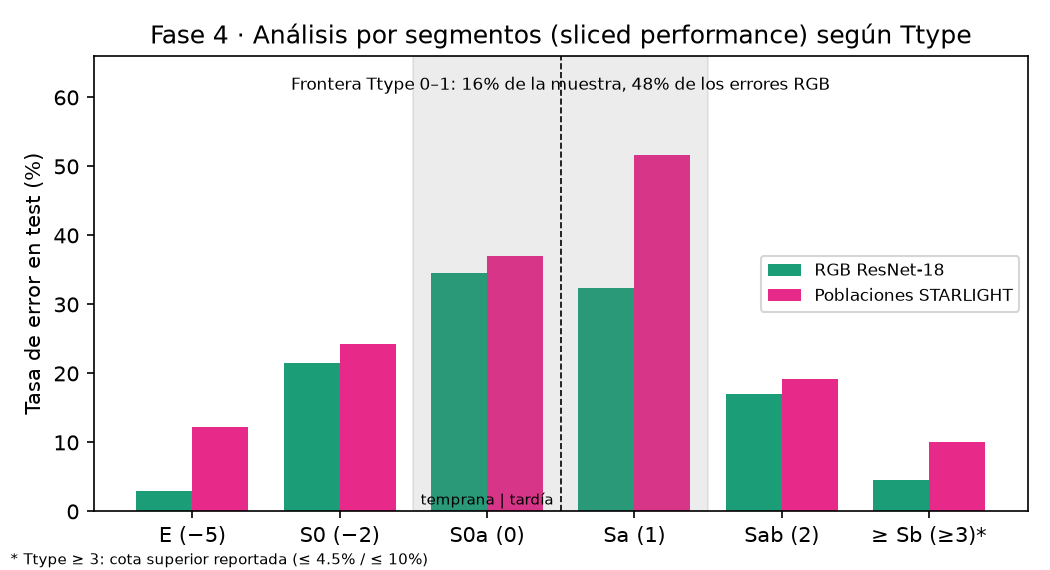
\includegraphics[width=0.83\linewidth]{fig3_error_por_ttype.png}
  \caption{Tasa de error según tipo morfológico. Los errores se concentran alrededor de la frontera entre las clases temprana y tardía.}
  \label{fig:error-ttype}
\end{figure}

El estudio de complementariedad halló que el modelo de poblaciones corregía 51.6\% de los 157 errores del baseline RGB (IC [43.7\%, 58.8\%]); se compartían 76 errores y el Jaccard entre conjuntos de errores era 0.25. Al menos uno de cuatro expertos secundarios corregía 64.3\% de los errores RGB. Un oráculo que escogiera, después de conocer la respuesta, cuál modelo acertó elevaría la exactitud de 0.888 a 0.946 (ganancia 0.058; IC [0.046, 0.068]); ese oráculo no es una política realizable. La fusión tardía con $\alpha^*=0.85$ produjo $\Delta$AUC de +0.0005 (IC [-0.0012, +0.0022]) y McNemar no indicó diferencia significativa (valores $p$ entre 0.14 y 1.0). La señal complementaria motiva nuevos experimentos, pero no justifica aún un gate de producción.

Además, 35 errores RGB (22.3\%) tuvieron alta confianza, definida como $|p-0.5| \geq 0.40$. Por tanto, la revisión no debe depender únicamente de seleccionar probabilidades cercanas a 0.5: conviene auditar periódicamente errores de alta confianza y los segmentos morfológicos problemáticos.

\section{Implementación y operación}

\subsection{Arquitectura propuesta}

La arquitectura siguiente describe una ruta futura de operación, no un sistema ya desplegado. El flujo empieza con imágenes y metadatos validados, aplica las transformaciones reproducibles y ejecuta la CNN versionada. Cada predicción debe conservar identificador, versión de datos y modelo, probabilidad, clase sugerida y marcas de calidad. La salida puede dirigirse a una cola de revisión humana según umbrales definidos con los usuarios científicos.

\begin{figure}[H]
\centering
\begin{tikzpicture}[
  node distance=0.65cm and 0.75cm,
  bloque/.style={draw,rounded corners,align=center,minimum height=0.85cm,text width=2.6cm,font=\small},
  ancho/.style={draw,rounded corners,align=center,minimum height=0.85cm,text width=3.0cm,font=\small},
  flecha/.style={-{Stealth[length=2mm]},thick}
]
\node[bloque] (datos) {Catálogos\\Legacy Survey / MaNGA};
\node[bloque,right=of datos] (validacion) {Ingesta y validación\\IDs, calidad, esquema};
\node[bloque,right=of validacion] (prep) {Preparación\\grz, recorte, normalización};
\node[bloque,right=of prep] (modelo) {Registro de modelos\\CNN versionada};
\node[bloque,right=of modelo] (infer) {Inferencia\\clase y probabilidad};

\node[ancho,below=of prep] (human) {Revisión experta\\casos inciertos / auditoría};
\node[bloque,left=of human] (salida) {Catálogo anotado\\predicción y trazabilidad};
\node[bloque,right=of human] (monitor) {Monitoreo\\calidad, deriva, métricas};

\draw[flecha] (datos) -- (validacion);
\draw[flecha] (validacion) -- (prep);
\draw[flecha] (prep) -- (modelo);
\draw[flecha] (modelo) -- (infer);
\draw[flecha] (infer) -- (human);
\draw[flecha] (human) -- (salida);
\draw[flecha] (infer) -- (monitor);
\draw[flecha] (monitor) -- (human);
\draw[flecha] (salida) -- (monitor);
\end{tikzpicture}
\caption{Arquitectura propuesta para inferencia controlada y revisión humana. La retroalimentación experta debe versionarse y no incorporarse al entrenamiento sin revisión.}
\label{fig:arquitectura}
\end{figure}

\subsection{Requisitos y responsables sugeridos}

La asignación de responsabilidades distingue a quienes definen el uso, aportan datos, diseñan y mantienen el sistema, y operan la plataforma, siguiendo la perspectiva de roles de stakeholders en proyectos de IA \parencite{miller2022}. Los responsables propuestos deben confirmarse con las instituciones participantes antes de desplegar.

\begin{table}[H]
\centering
\caption{Requisitos mínimos para una operación futura y responsables sugeridos.}
\label{tab:responsables}
\begin{tabularx}{\linewidth}{>{\raggedright\arraybackslash}p{3.1cm}X>{\raggedright\arraybackslash}p{3.2cm}}
\toprule
Requisito & Evidencia o control operativo & Responsable sugerido\\
\midrule
Gobernanza y uso & Definir propósito, población cubierta, política de revisión y usos no permitidos. & Patrocinadores científicos de IA-UNAM; responsables de decisión\\
Datos y permisos & Versionar catálogos, procedencia, licencias, selección, filtros y emparejamiento de identificadores. & Custodio de datos / equipo de datos MaNGA y Legacy\\
Preprocesamiento & Mantener código y parámetros para orientación, canales, FoV, resolución y normalización. & Equipo desarrollador; mantenedor del modelo\\
Modelo y artefactos & Versionar pesos, configuración, dependencias, métricas, particiones y predicciones de evaluación. & Mantenedor del modelo\\
Infraestructura & Proveer almacenamiento, cómputo, autenticación, registro de ejecuciones y respaldos. & Equipo de cómputo / TI de IA-UNAM\\
Validación científica & Revisar muestras, errores por tipo y cambios de dominio antes de liberar versiones. & Expertos en morfología; patrocinadores\\
Revisión humana & Definir umbrales, registrar decisiones y escalar objetos dudosos. & Usuarios científicos / equipo de análisis\\
\bottomrule
\end{tabularx}
\end{table}

Los experimentos ya producen artefactos útiles para trazabilidad, como configuración, historial de entrenamiento, resultados, predicciones y checkpoints. En un flujo productivo deben empaquetarse junto con la versión del código, el manifiesto de datos y las dependencias. La firma de una versión debe requerir una evaluación en datos separados y aprobación experta; un cambio de encuesta o instrumento no debe tratarse como una actualización transparente.

\subsection{Monitoreo y respuesta}

El monitoreo debe detectar cuándo cambia la distribución de entrada o deja de ser válida la relación entre imagen y etiqueta. No basta con vigilar la exactitud global, pues las etiquetas expertas nuevas llegan con retraso y un promedio puede ocultar degradaciones por subgrupo.

\begin{table}[H]
\centering
\caption{Señales de monitoreo y acciones ante desviaciones.}
\label{tab:monitoreo}
\begin{tabularx}{\linewidth}{>{\raggedright\arraybackslash}p{3.1cm}X>{\raggedright\arraybackslash}p{3.1cm}}
\toprule
Señal & Qué observar & Acción sugerida\\
\midrule
Calidad de imagen & \texttt{bright\_flag}, \texttt{line\_flag}, \texttt{is\_suspicious}, canales faltantes, orientación y saturación. & Poner en cuarentena lotes atípicos; revisar transformaciones.\\
Deriva de datos & Distribuciones de tamaño angular, $z$, colores, región norte/sur y versión de encuesta. & Comparar con entrenamiento; suspender extrapolaciones no validadas.\\
Calibración y confianza & ECE, Brier, histogramas de probabilidad y frecuencia de casos en banda de revisión. & Recalibrar o ajustar el punto operativo solo con datos etiquetados independientes.\\
Desempeño por clase y tipo & Matriz de confusión, recuperación por clase y error en \texttt{Ttype}=0--1. & Revisión científica focalizada; no depender solo de la métrica agregada.\\
Cambio de prevalencia & Proporción predicha de tempranas/tardías y distribución de puntajes. & Investigar cambios de población o de adquisición antes de reentrenar.\\
Servicio & Latencia, fallos de lectura, costo de cómputo y versiones de artefactos. & Alertar, restaurar una versión estable y conservar trazas.\\
\bottomrule
\end{tabularx}
\end{table}

Una señal de deriva por sí sola no prueba degradación: debe activar revisión de datos y, cuando se disponga de nuevas etiquetas expertas, evaluación de desempeño. La actualización del modelo debe usar una cohorte versionada, mantener una prueba temporal o externa y documentar el impacto sobre grupos relevantes. Cambios de DR11 a datos Rubin/LSST, de representación JPEG a FITS o de resolución requieren una validación de dominio explícita.

\section{Conclusiones clave}

La CNN compacta de imágenes fue el mejor clasificador final en la evaluación realizada: obtuvo AUC 0.9667, exactitud 0.8952 y exactitud balanceada 0.8980. Superó numéricamente al baseline ResNet-18 por 0.0034 de AUC y 0.0071 de exactitud, aunque el incremento de AUC es pequeño respecto de la incertidumbre y se observó en una sola partición. Ambos modelos superaron los umbrales establecidos de exactitud 0.829 y F1 0.83.

La decisión metodológica más importante fue no forzar la fusión multimodal como producto final. Las fusiones probadas no mejoraron de forma consistente a la imagen, y la variante de fusión final tuvo una diferencia de AUC significativamente negativa frente al control de imágenes en el bootstrap pareado. El análisis sí detectó complementariedad entre errores de imagen y poblaciones; convertirla en una política realizable requiere predicciones fuera de pliegue, evaluación independiente y un criterio de selección que no use la etiqueta verdadera.

La limitación central es la validez de las etiquetas: la morfología es una valoración experta, la división temprana/tardía impone una frontera convencional y los objetos cercanos a \texttt{Ttype}=0--1 concentran errores. Se añaden una sola semilla y partición, posible sesgo de selección por checkpoints, exploración descriptiva de la prueba durante el análisis de complementariedad, posible fuga norte/sur, calidad variable de imagen y la dependencia de STARLIGHT respecto de los mismos espectros. La exactitud a umbral 0.5 tampoco refleja necesariamente los costos de revisión ni la calibración en producción.

Como trabajo futuro se recomienda: (1) repetir la evaluación con múltiples semillas y validación externa o temporal; (2) obtener predicciones fuera de pliegue de cada experto y probar gates o stacking únicamente en validación; (3) analizar por separado objetos sospechosos, regiones y condiciones de imagen; (4) estudiar un esquema de etiquetas ordinal o revisión experta para la frontera morfológica; y (5) diseñar el flujo de producción con trazabilidad, umbrales de revisión humana y monitoreo de datos, calibración y errores por subgrupo. Hasta entonces, el clasificador debe considerarse un apoyo a la priorización científica, no un sustituto de la clasificación experta.

\section{Referencias y anexos}

\subsection*{Declaración de uso de inteligencia artificial}
Se utilizó una herramienta de inteligencia artificial como apoyo para sintetizar y redactar este documento. La selección de resultados, la verificación de cifras frente a los avances del proyecto y la responsabilidad sobre las conclusiones corresponden al equipo autor \parencite{anthropic2026claude}.

\printbibliography[heading=none]

\clearpage
\appendix
\section{Resultados complementarios}

\subsection{Comparación de candidatos}

\begin{table}[H]
\centering
\caption{Resultados de candidatos reportados en los experimentos de ablación. Las cifras corresponden a la partición de prueba del protocolo del proyecto.}
\label{tab:ablacion}
\begin{tabular}{lrr}
\toprule
Modelo & AUC & Exactitud\\
\midrule
ResNet-18 de imágenes (baseline) & 0.9633 & 0.8881\\
CNN de imágenes, corrida CPU & 0.9634 & 0.9009\\
CNN de imágenes, corrida GPU & 0.9623 & 0.9009\\
CNN de imágenes, FoV aleatorio & 0.9643 & 0.9002\\
Imagen + espectro FoV & 0.9635 & 0.8874\\
Imagen + espectro STARLIGHT & 0.9632 & 0.8931\\
Imagen + poblaciones & 0.9639 & 0.8988\\
Imagen + espectro + poblaciones & 0.9650 & 0.8895\\
MLP de poblaciones & 0.8949 & 0.8375\\
Espectro STARLIGHT + poblaciones & 0.8960 & 0.8346\\
CNN 1D de espectro FoV & 0.8572 & 0.7947\\
CNN 1D de espectro STARLIGHT & 0.8642 & 0.7890\\
CNN final de imágenes (Avance 5) & \textbf{0.9667} & \textbf{0.8952}\\
Fusión CNN + atención espectral (Avance 5) & 0.9334 & 0.8617\\
\bottomrule
\end{tabular}
\end{table}

Las cifras de distintas corridas no deben leerse como una búsqueda de máximo aislada del protocolo: la decisión final considera el diseño experimental, la estabilidad observada y el objetivo de simplicidad operativa. La corrida de CNN con FoV aleatorio de Avance 4 tuvo exactitud 0.9002, mientras que la configuración final de imagen reportó 0.8952; la elección final de Avance 5 corresponde a su control explícito de imágenes y a su comparación pareada con la fusión final.

\subsection{Diagnóstico de selección espectral}

En validación se observaron 257 desacuerdos entre expertos (18.3\%); el espectro fue el acertado en 33.1\% de esos desacuerdos. Un selector de confianza S2 obtuvo AUC OOF 0.676 (IC [0.604, 0.738], $p=0.005$), pero la ganancia neta estimada fue de solo 5 casos (IC [-9, 18]) frente a una ganancia oracle de 85. XGBoost presentó una brecha de 0.30 entre entrenamiento y OOF, compatible con sobreajuste. La conclusión fue que existe señal para investigar, pero no evidencia suficiente para justificar un gate operativo.

\subsection{Material gráfico reutilizado}

Las figuras referenciadas en el artículo se encuentran en \texttt{documents/entregables/avance/images/}. Al mantener el archivo \texttt{.tex} dentro de \texttt{documents/entregables/Articulo/}, las rutas definidas en \texttt{\textbackslash graphicspath} apuntan a esa carpeta. Entre las imágenes reutilizadas están \texttt{tipos\_galaxias.png}, \texttt{diag3\_flujo\_datos.png} y \texttt{fig3\_error\_por\_ttype.png}; pueden incorporarse otras del repositorio, como \texttt{fig2\_auc\_test.png}, \texttt{escala\_ttype.png} y \texttt{curvas\_entrenamiento.png}.

\end{document}
